\documentclass{article}
\usepackage{graphicx} 
\usepackage{multirow}
\usepackage{enumitem}
\usepackage{amssymb}
\usepackage{amsmath}
\usepackage{xcolor}
\usepackage{cancel}
\usepackage{tcolorbox}
\usepackage{physics}
\usepackage{geometry}
\usepackage{tikz}
\usepackage{tikz-3dplot}
\usepackage{pgfplots, tkz-euclide,calc}

\usetikzlibrary{angles,quotes} % for pic (angle labels)
\usetikzlibrary{arrows.meta}
\usetikzlibrary{calc}
\usetikzlibrary{decorations.markings}
\usetikzlibrary{bending} % for arrow head angle
\tikzset{>=latex} % for LaTeX arrow head
\usepackage{xcolor}
\pgfplotsset{compat=newest}

\colorlet{xcol}{blue!60!black}
\colorlet{myred}{red!80!black}
\colorlet{myblue}{blue!80!black}
\colorlet{mygreen}{green!40!black}
\colorlet{mypurple}{red!50!blue!90!black!80}
\colorlet{mydarkred}{myred!80!black}
\colorlet{mydarkblue}{myblue!80!black}
\tikzstyle{xline}=[xcol,thick,smooth]
\tikzstyle{width}=[{Latex[length=5,width=3]}-{Latex[length=5,width=3]},thick]
\tikzstyle{mydashed}=[dash pattern=on 1.7pt off 1.7pt]
\tikzset{
  traj/.style 2 args={xline,postaction={decorate},decoration={markings,
    mark=at position #1 with {\arrow{<}},
    mark=at position #2 with {\arrow{<}}}
  }
}
\def\tick#1#2{\draw[thick] (#1)++(#2:0.12) --++ (#2-180:0.24)}
\def\N{100} % number of samples
    \usetikzlibrary{patterns,snakes,shapes.arrows,3d}
    \usepgfplotslibrary{fillbetween}
	\geometry{
		total = {160mm, 237mm},
		left = 25mm,
		right = 35mm,
		top = 30mm,
		bottom = 30mm,
	}

\newcommand{\jawab}{\textbf{\underline{Solusi}}:}
\newcommand{\del}{\partial}
\newcommand{\cis}{\text{cis}}
\begin{document}
\setlength{\parindent}{0pt}
    \pagenumbering{gobble}
    \noindent
    \begin{tabular}{|lcl|}
     \hline
     Nama&:&Teosofi Hidayah Agung\\
     NRP&:&5002221132\\
     \hline
    \end{tabular}\\~\\
\noindent
    Tentukan solusi dari sistem persamaan diferensial berikut
    \[\dot{\vb*{x}}=\vb*{Ax},\quad\vb*{A}=\begin{bmatrix}
        2&-3\\
        1&2
    \end{bmatrix}\text{ dan }\vb*{x}=\begin{bmatrix}
        x\\
        y
    \end{bmatrix}\]
    dengan syarat awal $x(0)=1$ dan $y(0)=1$.\\
    \jawab\\
    Cari nilai eigen dari $\vb*{A}$
    \begin{flalign*}
        \det(\vb*{A}-\lambda\vb*{I})=\begin{vmatrix}
            2-\lambda&-3\\
            1&2-\lambda
        \end{vmatrix}=0&\iff\lambda^2-4\lambda+7=0&\\
        &\iff\lambda=\frac{4\pm\sqrt{16-28}}{2}&\\
        &\iff\lambda=2\pm\sqrt{3}i
    \end{flalign*}
    Kemudian cari vektor eigen dari $\vb*{A}$
    \begin{itemize}
        \item Untuk $\lambda_1=2+\sqrt{3}i$
        \begin{flalign*}
            (\vb*{A}-\lambda\vb*{I})\vb*{v_1}=\vb*{0}&\iff\begin{bmatrix}
                2-(2+\sqrt{3}i)&-3\\
                1&2-(2+\sqrt{3}i)
            \end{bmatrix}\begin{bmatrix}
                v_1\\
                v_2
            \end{bmatrix}=\begin{bmatrix}
                0\\
                0
            \end{bmatrix}&\\
            &\iff\begin{bmatrix}
                -\sqrt{3}i&-3\\
                1&-\sqrt{3}i
            \end{bmatrix}\begin{bmatrix}
                v_1\\
                v_2
            \end{bmatrix}=\begin{bmatrix}
                0\\
                0
            \end{bmatrix}&\\
            &\iff\begin{cases}
                -\sqrt{3}iv_1-3v_2=0\\
                v_1-\sqrt{3}iv_2=0
            \end{cases}&\\
            &\iff v_1=\sqrt{3}iv_2
        \end{flalign*}
        Sehingga vektor eigen untuk $\lambda=2+\sqrt{3}i$ adalah $\vb*{v_1}=\begin{bmatrix}
            \sqrt{3}i\\
            1
        \end{bmatrix}$.
        \item Untuk $\lambda_2=2-\sqrt{3}i$
        \begin{flalign*}
            (\vb*{A}-\lambda\vb*{I})\vb*{v_2}=\vb*{0}&\iff\begin{bmatrix}
                2-(2-\sqrt{3}i)&-3\\
                1&2-(2-\sqrt{3}i)
            \end{bmatrix}\begin{bmatrix}
                v_1\\
                v_2
            \end{bmatrix}=\begin{bmatrix}
                0\\
                0
            \end{bmatrix}&\\
            &\iff\begin{bmatrix}
                \sqrt{3}i&-3\\
                1&\sqrt{3}i
            \end{bmatrix}\begin{bmatrix}
                v_1\\
                v_2
            \end{bmatrix}=\begin{bmatrix}
                0\\
                0
            \end{bmatrix}&\\
            &\iff\begin{cases}
                \sqrt{3}iv_1-3v_2=0\\
                v_1+\sqrt{3}iv_2=0
            \end{cases}&\\
            &\iff v_1=-\sqrt{3}iv_2
        \end{flalign*}
        Sehingga vektor eigen untuk $\lambda=2-\sqrt{3}i$ adalah $\vb*{v_2}=\begin{bmatrix}
            -\sqrt{3}i\\
            1
        \end{bmatrix}$.\\
    \end{itemize}
    Sehingga solusi umum dari sistem persamaan diferensial adalah
    \begin{flalign*}
        \begin{bmatrix}
            x(t)\\
            y(t)
        \end{bmatrix}&=c_1\vb*{v_1}e^{\lambda_1t}+c_2\vb*{v_2}e^{\lambda_2t}\\
        &= c_1e^{(2+\sqrt{3}i)t}\begin{bmatrix}
            \sqrt{3}i\\
            1
        \end{bmatrix}+c_2e^{(2-\sqrt{3}i)t}\begin{bmatrix}
            -\sqrt{3}i\\
            1
        \end{bmatrix}&\\
        &=c_1e^{2t}\cis\left(\sqrt{3}t\right)\begin{bmatrix}
            \sqrt{3}i\\
            1
        \end{bmatrix}+c_2e^{2t}\cis\left(-\sqrt{3}t\right)\begin{bmatrix}
            -\sqrt{3}i\\
            1
        \end{bmatrix}
    \end{flalign*}
    Dengan syarat awal $x(0)=1$ dan $y(0)=1$, maka
    \begin{flalign*}
        &\begin{cases}
            \sqrt{3}ic_1-\sqrt{3}ic_2=1\\
            c_1+c_2=1
        \end{cases}&\\
        &\iff c_1=\frac{1}{2}-\frac{i}{2\sqrt{3}},\quad c_2=\frac{1}{2}+\frac{i}{2\sqrt{3}}&\\
    \end{flalign*}
    Sehingga solusi dari sistem persamaan diferensial adalah
    \begin{flalign*}
        \begin{bmatrix}
            x(t)\\
            y(t)
        \end{bmatrix}&=\left(\frac{1}{2}-\frac{i}{2\sqrt{3}}\right)e^{2t}\cis\left(\sqrt{3}t\right)\begin{bmatrix}
            \sqrt{3}i\\
            1
        \end{bmatrix}+\left(\frac{1}{2}+\frac{i}{2\sqrt{3}}\right)e^{2t}\cis\left(-\sqrt{3}t\right)\begin{bmatrix}
            -\sqrt{3}i\\
            1
        \end{bmatrix}&\\
    \end{flalign*}
    Sketsa kestabilan sistem adalah sebagai berikut
    \begin{center}
        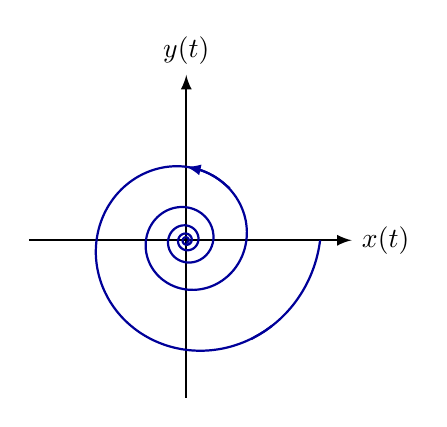
\begin{tikzpicture}
            \def\xmax{2.0}
            \def\A{1.7}
            \def\a{0.8}
            \def\ang{60}
            \def\T{0.5}  % decay constant tau
            \def\om{2.5} % decay constant tau
            \coordinate (O) at (0,0);
            \coordinate (X) at (\A,0);
            \draw[->,thick] (-\xmax,0) -- (\xmax+0.1,0) node[right] {$x(t)$};
            \draw[->,thick] (0,-\xmax) -- (0,\xmax+0.1) node[above] {$y(t)$};
            \draw[xline,samples=100,variable=\t]
              plot[domain=0:0.06]({\A*exp(-\t/\T)*cos(360*\om*\t)},{-\A*exp(-\t/\T)*sin(360*\om*\t)})
              --++ (-150:0.08);
            \draw[,xline,samples=100,variable=\t]
              plot[domain=0.05:0.34]({\A*exp(-\t/\T)*cos(360*\om*\t)},{-\A*exp(-\t/\T)*sin(360*\om*\t)})
              --++ (-40:0.08);
            \draw[<-,xline,samples=200,variable=\t] %,line cap=round
              plot[domain=0.3:2.1]({\A*exp(-\t/\T)*cos(360*\om*\t)},{-\A*exp(-\t/\T)*sin(360*\om*\t)});
            
            %\draw[->,mygreen!80!black] (-20:1.05*\A) arc(-20:-55:0.6*\A);

        \end{tikzpicture}
    \end{center}
\end{document}